\begin{comment}
\label{chapter:conceitos}
Este capítulo tem como objetivo apresentar os principais conceitos e definições abordados neste trabalho, tais como: Linguagens de descrição de hardware, Verificação de sistemas e Técnicas de Compiladores.

%============================
%Linguagens de descrição de hardware
%============================


\end{}
\section{Linguagens de descrição de hardware}

As linguagens de descrição de hardware(HDL) foram desenvolvidas com o intuito de auxiliar a criação de circuitos lógicos com grande número de elementos e com uma gama de abstrações lógicas e eletrônicas \cite{thomas2008verilog}. \textcolor{red}{Entre os exemplos, podemos citar: \textit{VDHL}, \textit{Verilog} e \textit{SystemC}.}

\par
Segundo \cite{christen1999vhdl}, linguagens de descrição de hardware são linguagens de programação utilizadas com o intuito de descrever o comportamento de um determinado circuito e processos, técnica conhecida como modelagem. Os modelos descritos em HDL são utilizados como entrada para um simulador, onde o mesmo pode ter seu comportamento analisado.

\begin{figure}[htb]
	\begin{center}
    \caption{\label{fig:waveform_fig}Waveform de multiplexador de duas entradas}
	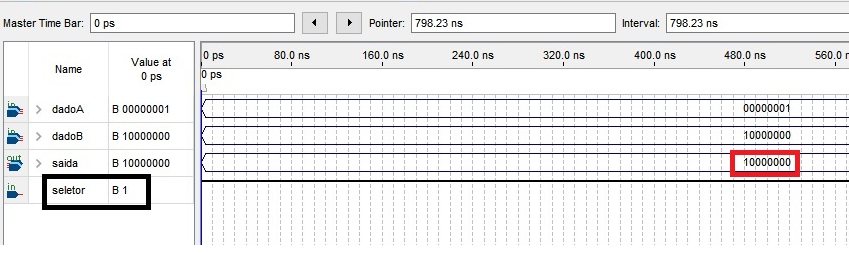
\includegraphics[scale=0.55]{Figuras/Waveform_multiplex.png}
	\end{center}
    \legend{Fonte: Própria}
\end{figure}

\par
As HDL's trazem consigo diversas vantagens, entre elas códigos independentes de tecnologia e fabricante, podendo ser portatéis e reutilizáveis\cite{cappelattipraticando}. As lingugens mais modernas, tais como VHDL e \textit{Verilog}, possuem suporte tanto a descrição do circuito propriamente dito quanto ao comportamento que o mesmo deve exercer\cite{christen1999vhdl}.

\par
\textcolor{red}{O \textit{Verilog}, como já citado, é uma linguagem de descrição de \textit{hardware} que fornece diversos níveis de abstração para desenvolvimento de sistemas digitais\cite{thomas2008verilog}. A linguagem foi desenvolvida para ser simples e efetiva nos diversos níveis de abstração incluindo o suporte ao desenvolvimento, verificação, síntese e testes de \textit{software}.\cite{IEEEVerilogLanguage}.}

\par
\textcolor{red}{O VHDL é uma linguagem de descrição de hardware amplamente utilizada concebida na década de 80, visto uma necessidade do Departamento de defesa dos Estados Unidos da América\cite{cappelattipraticando}. Assim como o Verilog, suporta desenvolvimento, verificação, síntese, e testes de \textit{hardware}\cite{IEEEVHDLLanguage}.}

\par
\textcolor{red}{Ambas as linguagens apesentam similaridades, sendo a linguagem VHDL escolhida para este projeto devido a linguagem apresentar maior gama de recursos tanto para o desenvolvimento quanto para oa auxilio nos testes.}\todo{O motivos da escolha ainda esta fraco, devido a familiaridades entre ambas as linguagens, ainda não sobre como colocar o motivo da escolha.}

%============================
%VHDL
%============================
\subsection{VHSIC Hardware Description Language - VHDL}\todo{Revisar textos e verificar a necessidade de mais exemplo}

VHDL é uma linguagem de descrição de hardware destina a ser utilizada em todas as etapas da criação de sistemas eletrônicos, sendo, desenvolvimento, verificação, síntese e teste de circuitos\cite{IEEEVHDLLanguage}.

\par
\textcolor{red}{Segundo \cite{cappelattipraticando}, o VHDL apresenta três principais pilares: Abstração, que consiste na descrição com diferentes níveis de detalhes; modularidade, que permite a divisão do projeto em vários blocos ou módulos para posterior interconexão; e hierarquia, permitindo que módulos ser compostos por submódulos e estes ter níveis de abstração diferentes, dependendo da necessidade do projeto. Devido a esta versatilidade que a linguagem VHDL foi selecionada para o projeto.}

\par
\textcolor{red}{Segundo \cite{IEEEVHDLLanguage}, é necessário um padrão para formatação da descrição em VHDL: \textit{Entity} (Pinos de entada/saída) e \textit{Architecture} (Arquitetura). A \textit{Entity} ou entidade representa o bloco onde são declaradas as entradas e as saídas do circuito utilizadas em todo o sistema, conforme apresentado na \autoref{fig:biblioteca_entidade}. A \textit{Architecture} ou arquitetura, apresentado na \autoref{fig:arquitetura}, define a relação entre entrada e saídas declaradas na entidade, podendo tais especificações serem completas ou parciais. Assim como em outras linguagens bibliotecas podem ser adicionadas, para que novos tipo possam ser utilizados no projeto.} 

\begin{figure}[thp]
\caption{\label{fig:biblioteca_entidade} Exemplo de declaração de bibliotecas e entidade.}
	\begin{center}
    \begin{minipage}{0.6\textwidth}
    \begin{lstlisting}       
library ieee;
use IEEE.STD_LOGIC_1164.ALL

ENTITY full_adder IS PORT(
	x1,x2,cin: in std_logic;
   S,count:out std_logic);
END full_adder;
\end{lstlisting}
    \end{minipage}
	\end{center}
    \legend{Fonte: Própria.}
\end{figure}

\begin{figure}[thp]
\caption{\label{fig:arquitetura} Exemplo de declaração da arquitetura no VHDL.}
	\begin{center}
    \begin{minipage}{0.6\textwidth}
    \begin{lstlisting}       
ARCHITECTURE behavioral OF full_adder IS
BEGIN
	s<=x1 XOR x2 XOR cin;
    cout<=(x1 AND x2) OR (x1 AND cin) OR (b AND cin);
END behavioral;

\end{lstlisting}
    \end{minipage}
	\end{center}
    \legend{Fonte: Própria.}
\end{figure}

\par
\textcolor{red}{Segundo \cite{cappelattipraticando},} uma descrição em VHDL pode conter diferentes níveis de abstração:
\begin{itemize}
  \item \textbf{Comportamental:} Permite descrever o circuito através de laços e processos. O circuito é definido em forma de um algoritmo, utilizando construção similares as utilizadas em linguagem de programação.
  
  \item \textbf{Transferencia de registradores:} Englobando a representação do dispositivo em nível de trasnferencia entre registradores, que consiste a utilização de funções lógicas combinacionais e registradores.
  
  \item \textbf{Estrutural:} O circuito é descrito mais próximo da implementação real, podendo ser definidas portas lógicas com atrasos unitarios ou com atrasos detalhados.
\end{itemize}

\todo[inline]{Tabala de caracteristicas do vhdl}

%============================
%PORTAS LÓGICAS
%============================
\subsection{Portas lógicas}

Segundo \citeauthor{idoeta1982elementos} conceito de portas lógicas é baseado na conhecida álgebra de Boole ou álgebra booleana, desenvolvida pelo matemático inglês George Boole em 1854. A álgebra booleana é representada por apenas dois valores, sendo eles o $0$ e $1$ e através disso expressar a relação entre entrada e saída dentro de um circuito. As portas lógicas podem ser construídas a partir de diodos, transmissões e resistores interconectados de modo que a saída seja o resultante de uma operação lógica básica realizada sobre as entradas \cite{tocci2003sistemas}. A figura \autoref{fig:algebra_booleana} apresenta um exemplo de álgebra booleana sem a utilização de diagramas.

\begin{figure}[htb]
	\begin{center}
    \caption{\label{fig:algebra_booleana}Exemplo de algebra booleana, onde A=0, B=1, C=1 e D=1.}
	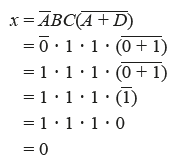
\includegraphics[scale=0.70]{Figuras/algebra_booleana.png}
	\end{center}
    \legend{Fonte: \cite{tocci2003sistemas}}
\end{figure}

\par
Ainda segundo \citeauthor{tocci2003sistemas}, devido a esta característica, a álgebra booleana possui três operações básicas, \texttt{OR} (ou), \texttt{AND} (e) e \texttt{NOT} (não). Tal conjunto de operações também é denominado de operações booleanas e via utilização de tabela-verdade é possível descrever as saídas baseando-se nas entradas e na operação aplicada. Cada operação booleana possui sua tabela verdade(\autoref{fig:exemplo_diagrama}), mas também sua representação em forma de diagrama.

\begin{figure}[htb]
	\begin{center}
    \caption{\label{fig:exemplo_diagrama}Simbolo e tabela verdade para uma porta OR de três entradas.}
	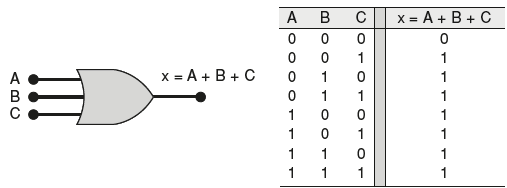
\includegraphics[scale=0.60]{Figuras/exemplo_diagrama.png}
	\end{center}
    \legend{Fonte: \cite{tocci2003sistemas}}
\end{figure}

\begin{figure}[htb]
	\begin{center}
    \caption{\label{fig:exemplo_circuito} Representação de circuito lógico, utilizando portas lógicas.}
	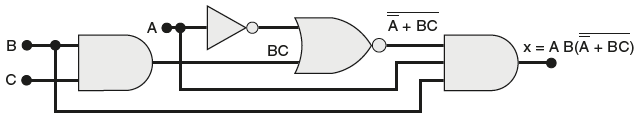
\includegraphics[scale=0.60]{Figuras/exemplo_circuito.png}
	\end{center}
    \legend{Fonte: \cite{tocci2003sistemas}}
\end{figure}

A \autoref{fig:exemplo_circuito} apresenta um circuito lógico formado pelas portas básicas da álgebra booleana. O circuito apresenta 3 entradas representadas pelas letras A, B e C, mas também formada por duas portas \textit{AND}, uma porta \textit{NOT} e uma porta \textit{OR}. Cada uma destas portas representando operações a serem realizadas, podendo receber como entrada um valor inicial ou resultante de outra porta, como no exemplo ocorre com a última porta \textit{AND}.

%============================
%VERIFICAÇÃO DE SISTEMAS
%============================
\section{Verificação de sistemas}
\textcolor{red}{ contexto inicial da verificação de sistemas, faz-se necessário o entendimento e a diferenciação entre verificação e validação. Verificação e validação possuem o intuíto de mostrar que determinado \textit{software} funcione conforme o especificado, além de satisfazer as especificações do cliente\cite{sommerville2011engenharia}.} 

\par
Segundo \cite{sargent2005verification}, Verificação é o processo de determinar se um modelo computacional obtido por discretização de um modelo matemático de um evento físico e o código que implementa o modelo computacional pode ser usado para representar o modelo matemático do evento com precisão suficiente e validação é o processo de determinar se um modelo matemático de um evento físico representa o evento físico real com precisão suficiente.

\par
\textcolor{red}{A verificação consite identificação de erros e provavéis problemas que um componente pronto possa apresentar, enquanto a validação busca analisar se tal componete esta seguindo os requisitos pré-definidos para sua construção\cite{koscianski2007qualidade}. O teste de programa, na qual o software  é executado com dados de teste é a principal forma de validação, porém, tecnicas de verificação, tais como, inspeção e revisões também podem integrar a etapa de validação\cite{sommerville2011engenharia}.}

\subsection{Diagrama de decisão binária}
Diagrama de decisão binária é um grafo aciclico para representação de funcões boolenas. Existe uma ordem total rigorosa na ocorrência de variáveis à medida que uma atravessa o grafo da raiz para a folha. Dado o exemplo,\autoref{fig:bdd_fig}, \textit{f=(a$\lor$b)$\land$(c$\lor$d)} e utilizando a ordenação de variavél a < b < c < d. Dada a atribuição de valores booleanos as variaveis a, b, c e d, pode-se decidir se a atribuição torna a fórmula verdadeira atravessando o início do gráfico na raiz e ramificação em cada nó. Definindo a,c e d = 1 e c = 0 leva a folha de rótulo 1, portanto, a fórmula é verdadeira para essa tarefa\cite{clarke1994model}.

\begin{figure}[htb]
	\begin{center}
    \caption{\label{fig:bdd_fig}Arvore de decisão binária}
	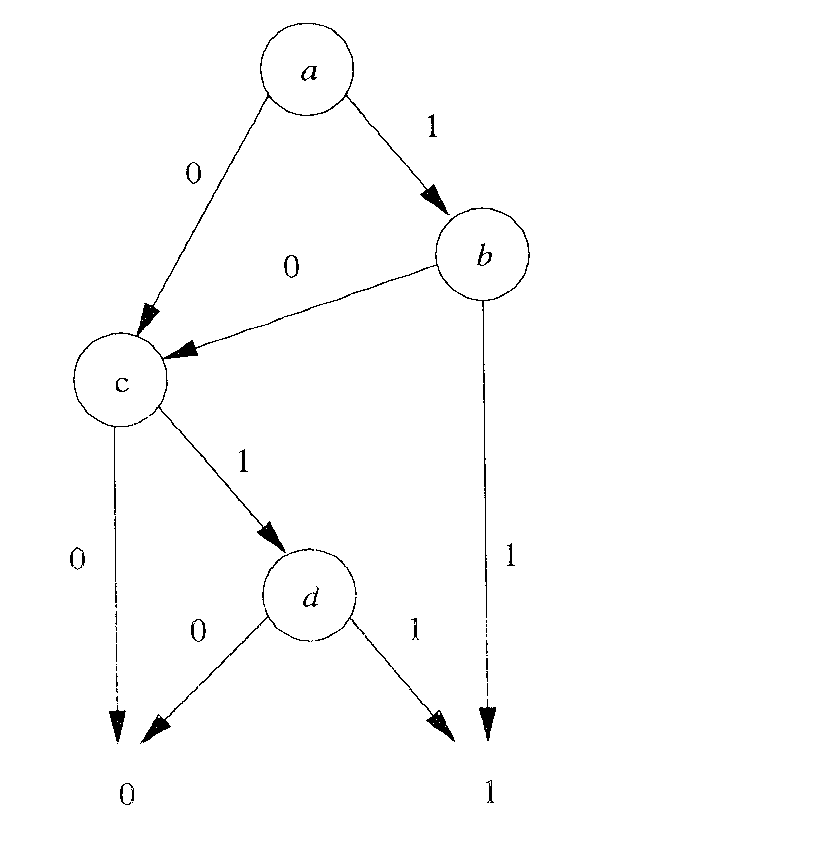
\includegraphics[scale=0.20]{Figuras/Arvore_BDD.png}
	\end{center}
    \legend{Fonte: \cite{clarke1994model}}
\end{figure}

%============================
%BOUNDED MODEL CHECKING
%============================
\subsection{\textit{Bounded Model Checking}}
Segundo, \citeauthor{rocha2015verificaccao}, \textit{Bounded Model Checking} (BMC) é um tipo especial de \textit{Model Checking} que geralmente utiliza o método de satisfabilidade booleana, o qual tem sido introduzido como uma técnica complementar para diagrama de decisão binaria para aliviar o problema da explosão de estados, visto que a técnica de \textit{Model Checking} busca todos os estados possíveis para verificação.

\par
Segundo \cite{rocha2015verificaccao} o \textit{Bounded Model Checking} é a verificação de uma propriedade especifica em uma determinada profundidade: dado um sistema de transições M, uma propriedade $\phi$, e um limite (\textit{bound}) $k$, o BMC desenrola o sistema $k$ vezes e traduz o sistema em uma condição de verificação(CV) $\psi$ tal que $\psi$ é satisfeito se e somente se $\phi$ tem um contra-exemplo de profundidade menor ou igual a $k$.

\par
O \textit{Extended SMT-Based Bounded Model Checker} (ESBMC) é um \textit{Bounded Model Checking} baseado em satisfabilidade booleana (SAT) que permite verificação aritmética de overflow e undeflow, segurança de ponteiros, limite de array, de gerar propriedades de segurança em programas em C/C$++$. ESBMC utiliza uma versão modificada do CBMC no \textit{front-end} para analisar o código ANSI-C e para gerar as condições de verificação através de execução simbólica \cite{cordeiro2012smt,rocha2015verificaccao}.

\par
No ESBMC, o programa analisado é modelado em um sistema de transição de estados, conforme a trupla: M=(S,R,$S_{0}$), o qual é gerado um grafo de controle de fluxo(GFC), onde S representa o conjunto de estados, R $\subseteq$ SxS representa as transições e S $\subseteq$ S representa o conjuto de estados iniciais. Um estado s $\in$ S consiste no valor do contador de programa(PC) e os valores de todas as variáveis dos programas. O estado inicial $S_{0}$ atribui o inicio do programa GFC ao PC, desta forma o ESBMC identifica as transições, conforme a formula lógica, $\gamma$=($S_{i}$,$S_{i+1}$) que captura as retrições sobre os valores correspondntes do PC e das variáveis do programa\cite{cordeiro2012smt}.

\par
Segundo o site da ferramenta, a ferramenta permite ao usuário indicar propriedades adicionais usando assertivas que também são verificadas. O ESBMC converte as condições usando diferentes técnicas de background para posteriormente passar para verificador SMT. Outra vantagem é a ferramenta permitir verificação de software single-thread e multi-thread.

%============================
%REDES DE PETRI
%============================
\subsection{Redes de petri}
Redes de petri são ferramentas de modelagem gráfica/matemática. Como ferramenta gráfica são utilizadas como comunicação visual, como fluxogramas, por exemplo e como ferramenta matemática podem configurar modelos matemáticos que regem o comportamento dos sistemas. A grade premissa desta ferramenta é descrever sistemas de processamento de informações caracterizados como concorrentes, assíncronos, distribuídos, paralelos, não deterministas e/ou estocásticos\cite{murata1989petri}.

\par
\textcolor{red}{ As redes de petri são compostas, conforme apresentado na \autoref{fig:rede_petri}, grafos direcionais compostos por nós e arcos. Os nós representam as transições e eventos e os arcos representam os pesos. Dentro desta representação, os arcos e eventos são componentes passivos enquanto as transições são ativos. A principal vantagem da utilização das redes de petri esta relacionado ao chamado "\textit{Token game}" que consiste no comportamento da rede de petri, em outras palavras, representa o funcionamento do sistema representado pela rede\cite{halder2006}.}

\begin{figure}[htb]
	\begin{center}
    \caption{\label{fig:rede_petri}Rede de petri}
	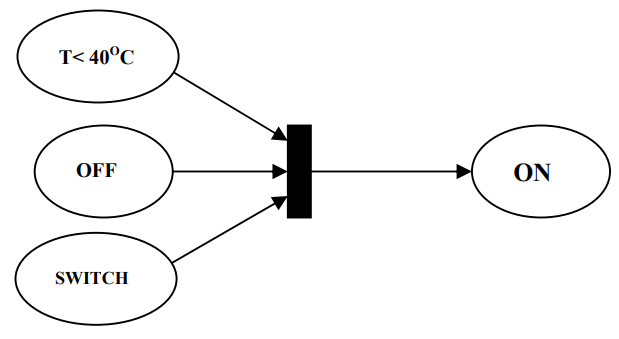
\includegraphics[scale=0.40]{Figuras/rede_petri.png}
	\end{center}
    \legend{Fonte: \cite{halder2006}}
\end{figure}
%============================
%VERIFICAÇÃO DE HARDWARE
%============================
\subsection{Verificação formal de hardware}

A verificação de hardware, por meio da simulação, via assegurar que uma implemetação, descrição do hardware em qualquer qualquer nível de abstração da hierarquia e hardware, atinja suas especificações, propriedades que devem ser respeitadas para que a corretude do mesmo seja comprovada \cite{gupta1992formal}. A Verificação formal de hardware consiste na utilização dos conceitos de verificação formal, mas também técnicas para corretude de circuitos lógicos, ou seja, consiste na utilização de modelos matemáticos para descrição de propriedade e/ou de comportamento de um dado sistema.\cite{kropf2013introduction}.

\par
\textcolor{red}{Entre as abordagens utilizadas verificação formal de hardware consiste em tanto a implementação quanto a especificação estarem descritas em lógica formal, neste caso a corretude será obtida através da comprovada relação entre a implementação e a especificação\cite{seger1992introduction}. A especificação formal consiste na descrição do comportamento, bem como, das propriedades do sistema em linguagem matemática, tornando-se crucial para o processo de verificação. Na implementação formal, o nível de abstração, tais como, \textit{Gate level} e RTL são importantes informações para o desenvolvimento do formalismo, bem como as classes, por exemplo se o circuito é sequencial ou combinacional, se utiliza pipeline, etc.\cite{kropf2013introduction}.}

\par
\textcolor{red}{A utilização de \textit{Model Checking} também se faz presente nos modelos formais de verificação de hardware, onde apenas é utilizado o comportamento dos circuitos na verificação, de modo a verificar a se as propriedades  presentes são satisfeitas. Para isso, são utilizados os conceitos da lógica proposicional, que por meio da utilização de fórmulas que representem as propriedades dos estados, é possível realizar as verificações necessárias\cite{seger1992introduction}.}
 
%============================
%VERIFICAÇÃO DE SOFTWARE
%============================
\subsection{Verificação formal de software}

Segundo \citeauthor{rocha2015verificaccao}, o uso de software tem sido feito em muitas áreas, tais como, infraestruturas industriais de missão critica e de segurança.  Logo, existe a necessidade de garantir a corretude destes sistemas. Devido a isso, a verificação formal tem sido utilizada em três principais abordagens, sendo elas~\cite{cousot2010gentle,d2008survey}:
\begin{itemize}
 \item \textcolor{red}{\textbf{Métodos dedutivos:} Produzem provas matemáticas formais de corretude usando provadores de teoremas ou assistentes de prova para execução da prova e necessitam da interação humana para prover os argumentos\cite{cousot2010gentle};}
  \item \textbf{Verificação de modelos:} Exploram exaustivamente modelos de execuções de programa, que podem ser sujeitos a explosão combinatória, necessário a intervenção humana para geração dos modelos.\cite{rocha2015verificaccao};
  \item \textcolor{red}{\textbf{Analise estática:} Engloba diversas técnicas para calcular automaticamente informações sobre o comportamento de um programa sem executá-lo, sendo utilizado em otimização de código e verificação em compiladres\cite{d2008survey}.}
\end{itemize}

Ainda segundo \citeauthor{rocha2015verificaccao}, na verificação formal apresentam-se dificuldades, tais como: quais as propriedades são de interesse na verificação no tempo de execução; e impossibilidade matemática de provar a corretude de propriedades não triviais no comportamento de programas, devido ao computador ser um dispositivo finito\cite{cousot2010gentle}. 

\todo[inline]{Sugiro adicionar um exemplo de verificacao de SW.}

%============================
%LÓGICA PROPOSICIONAL
%============================
\subsection{Lógica proposicional}
A lógica proposicional é uma linguagem formal onde é definida um alfabeto e conectivos proposicionais, e um conjunto de regras gramaticais, as quais serão utilizadas para construção das proposições\cite{souza2017logica}. Porém apesar de importante, ela é limitada, não podendo expressar sentenças elementares importantes, tais como a da aritmética elementar. Por exemplo:
\begin{enumerate}
\item Todos são mortais.
\item Alguém é bondoso.
\end{enumerate}
Na lógica preposicional, não poderiam ser analisadas, pois não teria como decompor ambas em sentença e assim não teria como analisar as diferenças entre ambas\cite{abe2002introducao}. Contudo, no exemplo:
\begin{enumerate}
\item Existem cavalos com patas verdes.
\end{enumerate}
A relação criada pela frase poderia  a ser analisada pela lógica proposicional\cite{abe2002introducao}.

Segundo \citeauthor{souza2017logica}, alfabeto da lógica proposicional é formado por símbolo de pontuação, símbolos proposicionais e conectivos proposicionais, onde cada um apresenta uma função em específico, sendo:
\begin{itemize}
\item \textbf{Símbolos de pontuação: }Apenas dois símbolos de pontuação são utilizados o "(" e o ")".
\item \textbf{Símbolos proposicionais:} São utilizados para representar as proposições, onde um símbolo \textit{P} pode ser utilizado para representar uma proposição qualquer, por exemplo: \textit{P}="Está chovendo". O conjunto de símbolos proposicionais é infinito e enumerável, sendo possível representar infinitos e enumerável conjunto de proposições.
\item \textbf{Conectivos proposicionais:} São os símbolos usando frequentemente na matemática. Os símbolos recebem a seguinte denominação: 
\begin{enumerate}
\item \textbf{$\neg$}: Representa a partícula de negação, ou seja, "Não".
\item \textbf{$\lor$}: Representa a partícula "Ou"
\item \textbf{$\land$}: Representa a partícula "E"
\item \textbf{$\rightarrow$}: Representa a partícula "Se então ou implica".
\item \textbf{$\Leftrightarrow$}: Representa a partícula "Se, e somente se".
\end{enumerate} 
\end{itemize}

Ainda segundo \citeauthor{souza2017logica}, existem as fórmulas que são constituídas de forma indutiva, a partir de símbolos do alfabeto conforme as regras apresentadas abaixo:
\begin{itemize}
\item Todo o símbolo preposicional é uma fórmula
\item Se \textit{H} é uma fórmula, então ($\neg$\textit{H}), a negação de \textit{H}, é uma fórmula.
\item Se \textit{H} e \textit{G} são fórmulas, então a disjunção de \textit{H} e \textit{G}, dada por (\textit{H} $\lor$ \textit{G}), é uma fórmula.
\item Se \textit{H} e \textit{G} são fórmulas, então a conjunção de \textit{H} e \textit{G}, dada por (\textit{H} $\land$ \textit{G}), é uma fórmula.
\item Se \textit{H} e \textit{G} são fórmulas, então a implicação de \textit{H} e \textit{G}, dada por (\textit{H} $\rightarrow$ \textit{G}), é uma fórmula. Neste caso, \textit{H} é o antecedente e \textit{G} consequente da fórmula.
\item Se \textit{H} e \textit{G} são fórmulas, então a bi-implicação de \textit{H} e \textit{G}, dada por (\textit{H} $\leftrightarrow$ \textit{G}), é uma fórmula. Neste caso, \textit{H} é o lado esquerdo e \textit{G} o lado direito da fórmula.
\end{itemize}


%============================
%Property Specification Language - PSL
%============================
\subsection{Linguagem de especificação de propriedades}
Linguagem de especificação de propriedades, do inglês \textit{Property Specification Language} - PSL, é uma notação formal para especificação de comportamento em sistemas eletrônicos, compatível com as linguagens VHDL, Verilog, SystemC e SystemVerilog. Destina-se a utilização para a especificação funcional, mas também para entrada de ferramentas de verificação. A especificação do PSL é a utilização de assertivas sobre propriedades de um sistema, sendo estas propriedades constituídas de três elementos: expressões boolenas, expressões sequenciais e operadores temporais\cite{IEEEPSL}.

\par
Segundo \cite{IEEEPSL}, o PSL foi totalmente desenvolvida com o intuito fornecer leitura e escrita de fácil entendimento, sintase concisa, semântica formal e rigorosamente bem definida e ser matematicamente precisa, visto a utilização da mesma em processo de verificação. Entre os pontos principais do PSL encontram-se:
\begin{itemize}
\item Sintaxe concisa,
\item Semântica formal rigorosamente definida,
\item Permite a especificação de propriedades reais,
\end{itemize}

\par
O PSL pode ser utilizado para capturar requisitos relativos ao comportamento total do projeto, bem como, sobre o modo que o mesmo deverá operar no ambiente, ms também para capturar requisitos comportamentais e os pressupostos que surgem durante o processo de design. Ambas podem ser utilizadas para verificação de sistemas \cite{IEEEPSL}.
%============================
%Assertion-based verification - ABV
%============================
\subsection{Verificação baseada em assertivas}
Verificação baseada em assertivas, do inglês\textit{Assertion-based verification} - ABV, é um paradigma de verificação igualente adequado para verificação formal e abordagens baseadas em simulação\cite{boule2005incorporating} e em conjunto com a tecnica de PSL tem ganhado aceitação como um método essencial para verificação funcional do hardware\cite{DahanCombining}.

\par
A técnica utiliza assertivas, que são declaração adicionadas ao projeto com o intuito de especificar o comportamento do projeto, podendo escritos em PSL ou em SVA(\textit{System Verilog Assertions.}\cite{boule2005incorporating}. No caso deste projeto será utilizado a PSL, devido a mesma ser utilizada juntamente com a linguagem VHDL.

\par
Com o ABV e as assertivas, circuito pode ser verificado usando técnicas de simulação e/ou verificação, por exemplo, \textit{Model Checking}, para garantir que o mesmo esteja de acordo com o pretendido co projeto\cite{DahanCombining}. 

Na \autoref{fig:assertiva} apresenta o modelo de assertiva utilizada no projeto, utilizando de um modelo próprio para assertivas, unindo as funcionalidades já existentes nas assertivas do VHDL, mas também novas, fornecendo assim mais propriedades a serem analisadas.

\begin{figure}[thp]
\caption{\label{fig:assertiva} Exemplo de declaração de assertiva no VHDL.}
	\begin{center}
    \begin{minipage}{0.9\textwidth}
    \begin{lstlisting}       
library ieee;
use ieee.std_logic_1164.all;

entity AND_ent is
port(   x,y: in bit;
        F: out bit
);
end AND_ent;

architecture behav1 of AND_ent is
begin
	--@c2vhdl:ASSERT
    --assert not (x='0' and y='1')
    --report "Both values of signals x and y are equal to 1"
    --severity ERROR;
    --@c2vhdl:END

	process(x, y)
    	begin
        	if ((x='1') and (y='1')) then
            	F <= '1';
        	else
            	F <= '0';
        	end if;
    	end process;4
end behav1;

\end{lstlisting}
    \end{minipage}
	\end{center}
    \legend{Fonte: Própria.}
\end{figure}
%============================
%PROPRIEDADES DE SEGURANÇA
%============================
\subsection{Propriedades de segurança}
Propriedades de segurança é um meio de validação do comportamento de um determinado sistema, de modo que ser uma propriedade de segurança for violada, então através de uma execução finita, é possível verificar tal erro. Algumas propriedades de segurança, no entanto, podem impor requisitos em fragmentos de caminho finito e não podem ser verificadas considerando apenas os estados alcançáveis. \cite{baier2008principles}.

\par
Segundo \cite{clarke2003verification}, podemos definir uma propriedade de segurança como: \textit{dado um sistema de transições $ST = (S, S_0, E)$, seja um conjunto $B \subset S$ que especifica um conjunto de maus estados tais que $S_0 \cap B = \emptyset$, pode-se dizer que $ST$ é seguro com relação a $B$, denotado por $ST \models AG\neg B$ se não existe um caminho no sistema de transição do estado inicial $S_0$ até o estado $B$, de outro modo é dito que $ST$ não é seguro}.
%============================
%TECNICAS DE COMPILADORES
%============================
\section{Técnicas de compiladores}
\par
Compiladores são sistemas de software utilizados para tradução de uma linguagem de programação para outra, ou seja, o programa da linguagem fonte é lido e traduzido para um código equivalente na outra linguagem, ou linguagem alvo. Geralmente utilizada para transformar trechos de código em uma linguagem a ser executada pelo computador\cite{aho2007compilers}. 

\par
Diversas técnicas podem ser utilizadas nas diversas etapas, até que o código seja traduzido, tais como LL(1) e LR na análise sintática e \textit{Peephole} na otimização de código\cite{aho2007compilers}. Neste projeto serão focados as áreas de transformações de código e otimização de código.
%============================
%TRANSFORMAÇÕES DE CÓDIGO
%============================
\subsection{Transformações de código}
\par
\textcolor{red}{Transformações de código correspondem a uma complexa função que envolve analise de fluxo de dados e modificação completa do programa e são parte integral da alta performance e sistemas computacionais. Podem ser classificados em transformações escalares que reduzem o número de instruções a serem executadas no programa ou transformações paralelas que maximizam o paralelismo.\cite{srikant2002compiler}}

\par
\textcolor{red}{A \autoref{fig:cod_vhdl} representa o trecho de código apresentado na \autoref{fig:assertiva}. O trecho representa o comportamento das entradas, neste caso de um código da porta AND. E a figura \autoref{fig:cod_c} representa a tradução deste trecho em código na linguagem C. Esta tradução foi realizada pela ferramenta V2C, utilizada neste projeto.}

\begin{figure}[thp]
\caption{\label{fig:cod_vhdl} Trecho de código em VHDL representando porta AND.}
	\begin{center}
    \begin{minipage}{0.9\textwidth}
    \begin{lstlisting}       
	process(x, y)
    	begin
        	if ((x='1') and (y='1')) then
            	F <= '1';
        	else
            	F <= '0';
        	end if;
    	end process;
\end{lstlisting}
    \end{minipage}
	\end{center}
    \legend{Fonte: Própria.}
\end{figure}

\begin{figure}[thp]
\caption{\label{fig:cod_c} Trecho de código traduzido para linguagem C.}
	\begin{center}
    \begin{minipage}{0.9\textwidth}
    \begin{lstlisting}       
   /* Start of Translation */
   /* p0: */
   if (chg[x] || chg[y]) {
      if (((old[x]==1) && (old[y]==1))) {
      	new[f]=1;
      }
      else {
      	new[f]=0;
      }
   }
   /* End of Translation */

	\end{lstlisting}
    \end{minipage}
	\end{center}
    \legend{Fonte: Própria.}
\end{figure}
%============================
%OTIMIZAÇÃO ok
%============================
\subsection{Otimização de código}
\par
A otimização de código \textcolor{red}{consiste na melhoria do código intermediário gerado pelos algoritmos de compilação com o objetivo de rodar mais rapidamente, porém outros fatores podem ser introduzidos, como algoritmos menores.} Este fato não implica em afirmar que o melhor código é gerado, visto que dada a complexidade, raramente pode ser obtido que o código gerado pode ser o melhor possível\cite{aho2007compilers}.

\par
\textcolor{red}{Segundo \cite{aho2007compilers}, otimização local de código consiste na otimização de um bloco básico de código, ou seja, a otimização ocorre em um trecho especifico de código. Os blocos básicos são trecho onde não ocorrem saltos ou \textit{loops}, para nenhuma outra parte do código. A otimização global de código é baseado na analise do fluxo de dados, de modo que ocorra as elminação de instruções não necessárias ou substituição mais facil. A otimização global consite na analise completa do código.}

%============================
%Grafo Acliclico Direcional - GAD ok
%============================
\subsubsection{Grafo Acliclico Direcional - GAD}
\par
\textcolor{red}{Grafo Aciclico Direcional é utilizado para diversos fins dentro da estrutura de compiladores, principalmente para geração da parse tree otimização de código. Pode ser usado na representação de instruções unicas blocos básicos de código\cite{aho2007compilers}. O uso de GAD permite a melhoria de de código, tais como:
\begin{itemize}
\item Elminação de subexpressões locais comuns, ou seja, expressões que o valor já foi computado anteriomente;
\item Eliminação de código morto;
\item  Reordernamento de declarações buscando reduzir o tempo que o valor temporário necessita ser preservado em um registro;
\end{itemize}}

\par
\begin{figure}[thp]
\caption{\label{fig:basic_block} Exemplo de bloco basico de código.}
	\begin{center}
    \begin{minipage}{0.9\textwidth}
    \begin{lstlisting}
    a = b + c
    b = a - d
    c = b + c
    d = a - d
	\end{lstlisting}
    \end{minipage}
	\end{center}
    \legend{Fonte: \cite{aho2007compilers}}
\end{figure}

\begin{figure}[htb]
	\begin{center}
    \caption{\label{fig:gda}GAD do bloco básico da \autoref{fig:basic_block}}
	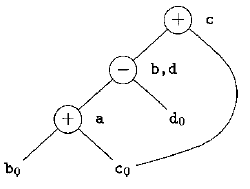
\includegraphics[scale=0.40]{Figuras/GDA.png}
	\end{center}
    \legend{Fonte: \cite{aho2007compilers}}
\end{figure}

\textcolor{red}{Na \autoref{fig:basic_block} apresenta um bloco básico com algumas instruções, no caso aresentando 4 operações entre somas e multiplicação e a partir deste bloco a \autoref{fig:gda} apresenta o GDA deste trecho de código. Nele aprsenta cada nó como uma operação especifica e os terminais como as parcelas das operações.}

%============================
%Grafo de Fluxo de Controle - GFC 
%============================
\subsubsection{Grafo de Fluxo de Controle - GFC}
\par
\textcolor{red}{Grafo de fluxo de controle corresponde a um grafo direcionado, no qual cada nó representa blocos básicos e cada aresta representa os caminhos de fluxo entre os blocos basicos.\cite{allen1970control}. É importante ressaltar que saltos determinam o final de um determinado bloco básico, ou seja, saltos indicam um caminho para uma nova região de código básico.\cite{aho2007compilers}.}


%============================
%Eliminção de código morto 
%============================
\subsubsection{Eliminção de código morto}
\par
\textcolor{red}{Elimincação de código morto é uma técnica busca a eficiência de um programa evitando a execução de instruções não necessária no tempo de execução.\cite{knoop1994partial}. Código morto consiste em instruções que não serão alcançáveis durante o fluxo do programa, sendo esta técnica basicamente a a retirada de qualquer variável que não será utilizada em qualquer outro nó do grafo\cite{aho2007compilers}.}

\par
\textcolor{red}{A utilização de GAD corresponde na eliminação de qualquer nó raiz, ou seja, nó sem ancestrais, as quais não esteja ativa anexada a mesma. A execução repetida desta operação removerá todos os nós correspondentes a código morto\cite{aho2007compilers}.}

\begin{figure}[htb]
	\begin{center}
    \caption{\label{fig:elimicacao_codigo}GAD do bloco básico da \autoref{fig:basic_block}}
	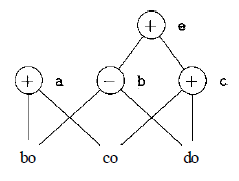
\includegraphics[scale=0.70]{Figuras/eliminacao_codigo.png}
	\end{center}
    \legend{Fonte: \cite{aho2007compilers}}
\end{figure}

\textcolor{red}{Na \autoref{fig:elimicacao_codigo}, supondo que os nós a,b e c estejam ativa, porém o nó é não esteja, o ultimo pode ser eliminado imediatamente. Os nós restantes continuam no GDA, a menos que não tenho variáveis ativas atreladas aos nós\cite{aho2007compilers}.}
%============================
%Analise do fluxo de dados ok
%============================
\subsubsection{Analise do fluxo de dados}
\par
\textcolor{red}{Analise de fluxo de dados refere-se ao conjunto de tecnicas que derivam informaçoes sobre o fluxo de dados ao longo dos caminhos de execução do programa. Para analise do programa, é necessário considerar todas as posiveis execuções através do grafo de fluxo.\cite{aho2007compilers}.}

%============================
%Gerador de código ok
%============================
\subsubsection{Gerador de código}
\par
O gerador de código é responsavél pela tradução final do programa-fonte para o programa-alvo, o mesmo recebe como entrada um código intermediário juntamente com a tabela de símbolos.Faz-se necessário que o programa-fonte tenha sido analisado sintatica e lexicamente, assim evitando que erros possam ser passados para o programa-alvo, por outro lado a existencia de uma nível de otimização, faz-se opicional neste caso\cite{aho2007compilers}.

\par
\textcolor{red}{O gerador de código possui três tarefs primarias, sendo as mesmas seleção de instrução, alocação de registros e atribuições. A seleção de instruções envolve a escolha das instruções apropriadas da máquina-alvo para implementar as declarações do código intermediario. A atribuição e atribuição de registros envolve a decisão sobre os valores a serem registrados nos registros\cite{aho2007compilers}.}

\end{comment}

\label{chapter:conceitos}


